\subsection{Gesamt Entropie und Entropie der Wurzel Wind}

\begin{figure}[H]
  \centering
  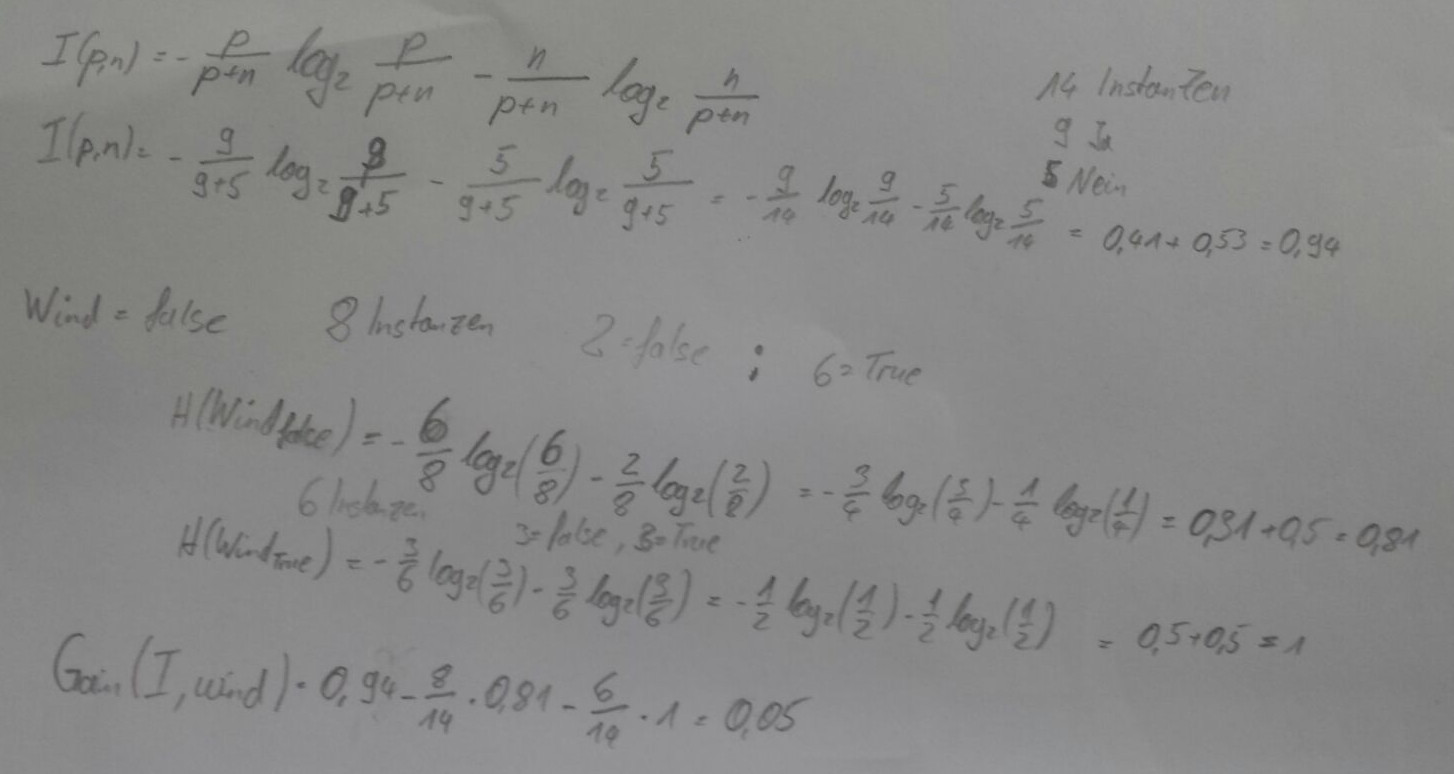
\includegraphics[height=9cm]{A3.jpeg}
\end{figure}

\subsection{Informationgewinn in abhängigkeit von verschiedenen Schniten}
Der Informationsgewin der verschiedenen Schnitte ist der Phythondatei zu entnehmen. Jedoch trat bei uns auf, das der Logarhytmus aus 0 gezogen werden musste. Deshalb konnte kein vernünfitger Gain aufgestellt werden.
